\section{Overview}
\label{sec:Overview}
\begin{figure*}[h!]
    \centering
    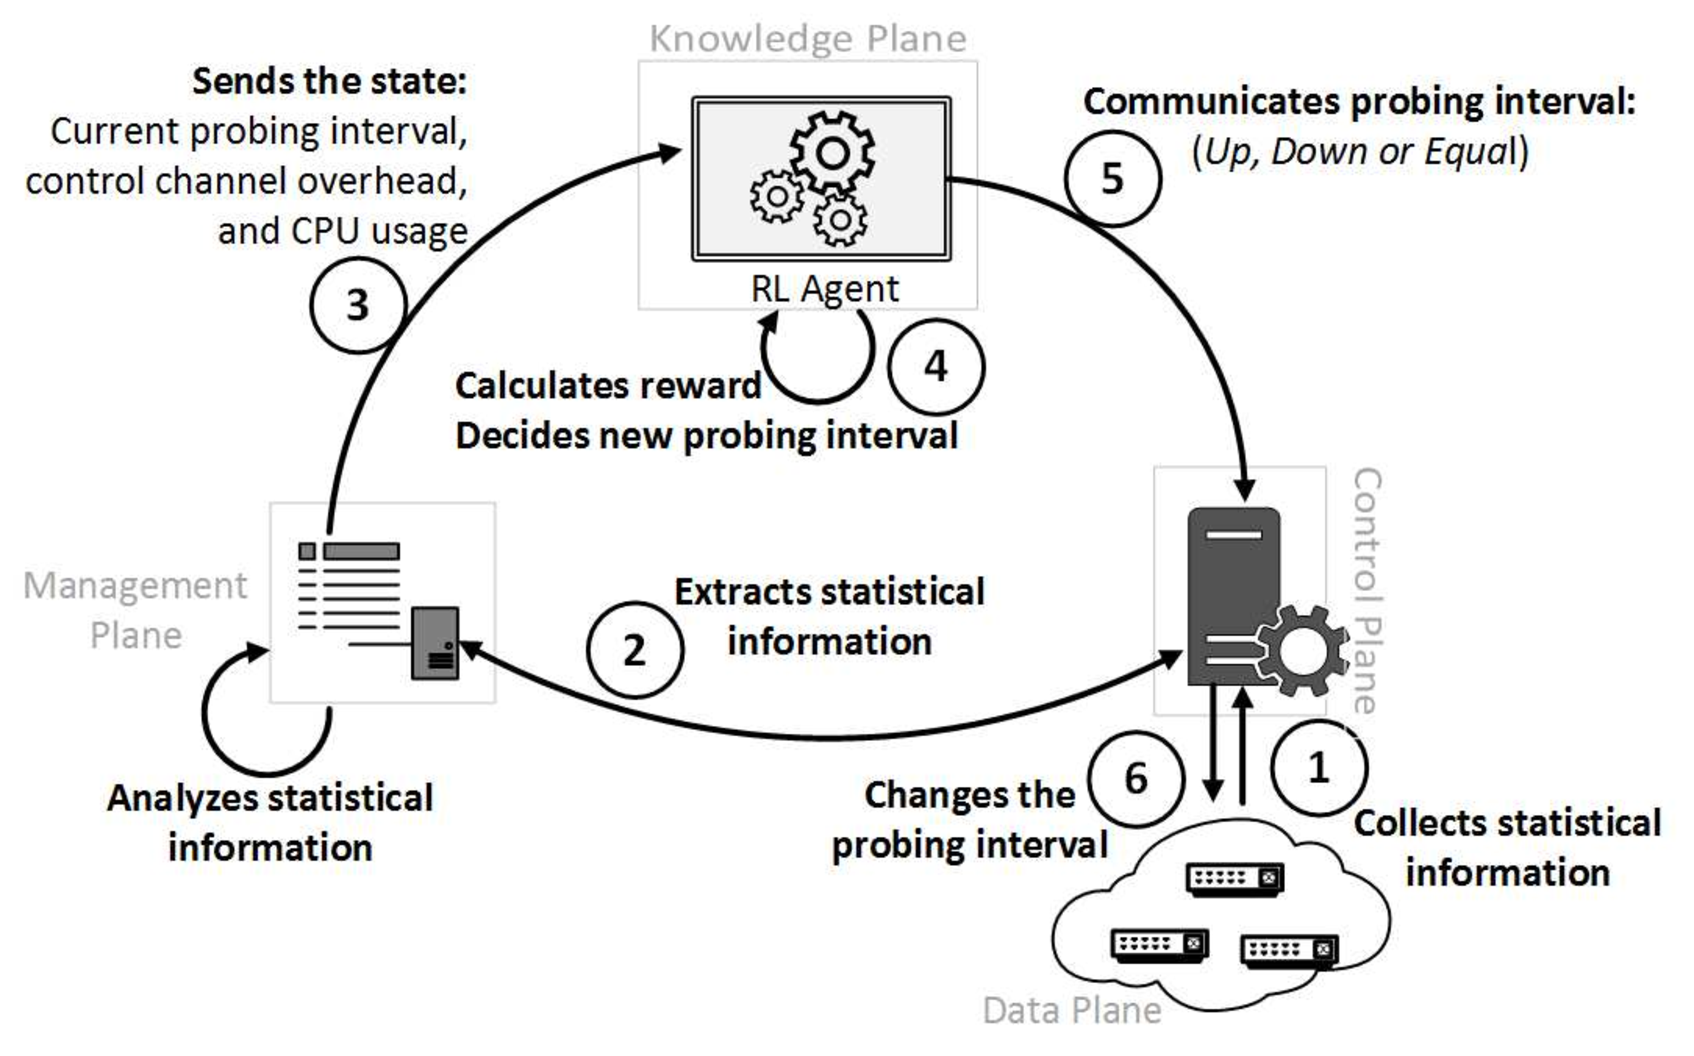
\includegraphics[width=0.75\textwidth]{figures/Figure2-IPro-high-level-operation}
    \caption{IPro - High-Level Operation}
    \label{fig:high_level_ipro}
\end{figure*}

IPro applies RL to optimize the probing interval regarding to CCO and CUC. Figure~\ref{fig:high_level_ipro} depicts how IPro operates in a high-abstraction level:

\begin{enumerate}[label=\protect\circled{\arabic*}]
    \item The Control Plane (CP) collects statistical information from the Data Plane (DP) at some probing interval. Since this collection of information affects the network behavior, the network falls in a new state.
    \item The Management Plane (MP) extracts these statistics to determine such a new state by analyzing CCO and CUC.
    \item MP sends this new state to the Knowledge Plane (KP).
    \item The RL-agent takes such a state to calculate the reward. It is important to highlight that a low reward indicates high CCO and high CUC. Based on the reward, the RL-agent decides a new probing interval intended to minimize CCO and CUC.
    \item The RL-agent communicates this new probing interval to CP.
    \item The CP applies this interval that affects the network behavior again. This operation continues until the network administrator decides to stop IPro.
\end{enumerate}

%\circled{1} the Control Plane (CP) collects statistical information from the Data Plane (DP) at some probing interval. Since this collection of information affects the network behavior, the network falls in a new state. \circled{2} the Management Plane (MP) extracts these statistics to determine such a new state by analyzing CCO and CUC. Subsequently, in \circled{3}, MP sends this new state to the Knowledge Plane (KP). In \circled{4}, the RL-agent takes such a state to calculate the reward. It is important to highlight that a low reward indicates high CCO and high CUC. Based on the reward, the RL-agent decides a new probing interval intended to minimize CCO and CUC. \circled{5} the RL-agent communicates this new probing interval to CP. In \circled{6}, CP applies this interval that affects the network behavior again. This operation continues until the network administrator decides to stop IPro.
